\documentclass[twocolumn,10pt]{article}
\title{Properties of shapes 1}
\setlength{\columnsep}{20pt} 
\usepackage{amsmath,hyperref,cancel,graphicx}
 \def\shrinkfactor{0.55}
 \usepackage[margin=1.5cm]{geometry}
\usepackage[usenames,dvipsnames]{color}
 
 \newcommand{\blue}[1]{{\color{Blue}#1}} 
 \newcommand{\purple}[1]{{\color{Purple}#1}} 
 \newcommand{\red}[1]{{\color{Red}#1}} 
 \newcommand{\green}[1]{{\color{Green}#1}} 
 \newcommand{\gray}[1]{{\color{Gray}#1}} 
  \newcommand{\pink}[1]{{\color{Magenta}#1}}   


\begin{document}
\maketitle



\section{\href{https://www.khanacademy.org/devadmin/content/items/x069890682ea2148d}{x069890682ea2148d}}

\noindent
**Which side is parallel to side $\overline{AE}$?**


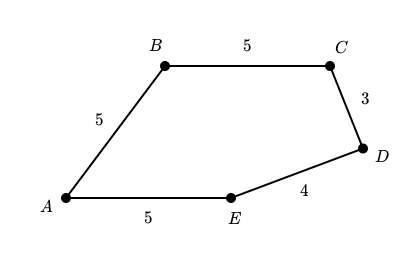
\includegraphics[scale=\shrinkfactor]{figures/0b1f52e2d56a98d5ec5f552c02f22f067ec40078.png}

\paragraph{Ans} Side [[? expression 1]] is parallel.
  BC

\paragraph{Hint 1}Parallel lines always remain the same distance apart and therefore never intersect. 

\paragraph{Hint 2}
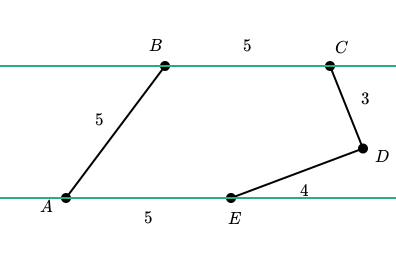
\includegraphics[scale=\shrinkfactor]{figures/83c724a031b6ec05f29446ad771043b503b36466.png}

\paragraph{Hint 3}Side $\overline{BC}$ is parallel to side $\overline{AE}$.



\medskip
\noindent
\textbf{Tags:} {\footnotesize CC.4.G.A.2, Properties of shapes 1, SB.4.1.L.4.TE, SB.4.1.L.4.CR, SB.4.1.L.5.TE}\\
\textbf{Version:} aeca907d.. 2013-10-11
\smallskip\hrule





\section{\href{https://www.khanacademy.org/devadmin/content/items/x134da82dcae224f9}{x134da82dcae224f9}}

\noindent
**Why are these shapes categorized into Group One and Group Two?** 

Group One 



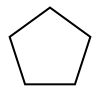
\includegraphics[scale=\shrinkfactor]{figures/498a6b09730fdba2360826c138eeee142e8cccc1.png}

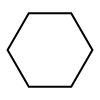
\includegraphics[scale=\shrinkfactor]{figures/0245164f3f4897772e76d361f955075a80732b03.png}

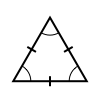
\includegraphics[scale=\shrinkfactor]{figures/2e6355867a1027528f1719f9dcb578dcb221b055.png}


Group Two


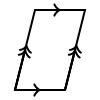
\includegraphics[scale=\shrinkfactor]{figures/feaa75a1e077e1d8ea6873bc2a4aa206d3c95598.png}

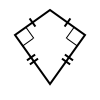
\includegraphics[scale=\shrinkfactor]{figures/be0b4c8e85edc438c12910c91d66875e8fcd2372.png}

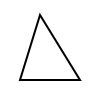
\includegraphics[scale=\shrinkfactor]{figures/ee7f87a00acb47dec4f2b2eed9a6741b21afc47d.png}



\paragraph{Ans} 

One group has parallel lines but the other does not.

\fbox{ One group has only equilateral shapes and the other has only shapes that are not equilateral.

}

 One group has shapes with four sides and the other has shapes that are not four sides.

One group has perpendicular lines but the other does not.



\paragraph{Hint 1}Parallel lines always remain the same distance apart and therefore never intersect.  Look at the pair of parallel lines below.  No matter how far they are extended, they will never meet.

$\phantom{xxxx}$

\includegraphics[scale=\shrinkfactor]{figures/7cf1fbfb7516a57d37ad80007a3886c81c33f393.png}  

Both groups have shapes that have parallel lines and shapes that don't have parallel lines.

\paragraph{Hint 2}Both groups have shapes that are not four sides (both have triangles).

\paragraph{Hint 3}Perpendicular lines intersect at a $90 ^\circ$ angle.
A right angle is in the shape of a perfect corner, like the corner of a typical sheet of paper.  Only one shape in the second group has perpendicular lines.

\paragraph{Hint 4}Equilateral shapes have sides of equal lengths.  The sides of the hexagon, the pentagon and the triangle are each equal.

\paragraph{Hint 5}The first group has only equilateral shapes and the second group has only shapes that are not equilateral.



\medskip
\noindent
\textbf{Tags:} {\footnotesize CC.4.G.A.2, Properties of shapes 1, SB.4.1.L.4.TE, SB.4.1.L.4.CR, SB.4.1.L.5.TE}\\
\textbf{Version:} 72c7bd77.. 2013-10-14
\smallskip\hrule





\section{\href{https://www.khanacademy.org/devadmin/content/items/x16d30b6ecc9d46ba}{x16d30b6ecc9d46ba}}

\noindent
**Put the shapes into the correct categories.**

[[? categorization 1]]


\paragraph{Ans} Drag and drop each card into the appropriate category. 

\paragraph{Hint 1}Parallel lines always remain the same distance apart and therefore never intersect.  Look at the pair of parallel lines below.  No matter how far they are extended, they will never meet.

$\phantom{xxxx}$

\includegraphics[scale=\shrinkfactor]{figures/7cf1fbfb7516a57d37ad80007a3886c81c33f393.png}

\paragraph{Hint 2} Perpendicular lines intersect at a $90 ^\circ$ angle.  
A right angle is in the shape of a perfect corner, like the corner of a typical sheet of paper.


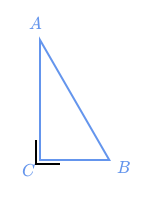
\includegraphics[scale=\shrinkfactor]{figures/497661f48f441186b5e021d8ca8c4f0c7449214f.png}

\paragraph{Hint 3}Parallel lines only:

$\phantom{xxxxxxxx}$
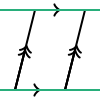
\includegraphics[scale=\shrinkfactor]{figures/dc97e97ad57144cae5a8b5bfdc5d541d8d66aa00.png}

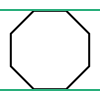
\includegraphics[scale=\shrinkfactor]{figures/f73cb50d59bdab17965cbcf6a6832a26002948cb.png}  
$\phantom{xxxxxxxx}$
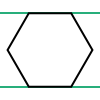
\includegraphics[scale=\shrinkfactor]{figures/a8914ec8b688d03af4fc47bdfdb83edcce453d65.png}

Perpendicular lines only:

$\phantom{xxxxxxxx}$
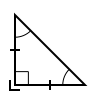
\includegraphics[scale=\shrinkfactor]{figures/f9413d967bb68c6b85d95672324c0a5b08af982e.png}

Both parallel and perpendicular lines:

$\phantom{xxxxxxxx}$
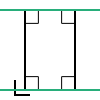
\includegraphics[scale=\shrinkfactor]{figures/ad42bf00e54b665d02d6e9aa787d9d04875ccc6e.png}

$\phantom{xxxxxxxx}$
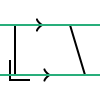
\includegraphics[scale=\shrinkfactor]{figures/c755ceca3f49cc6303844bb5cd33f40647ddfab0.png}



\medskip
\noindent
\textbf{Tags:} {\footnotesize CC.4.G.A.2, Properties of shapes 1, SB.4.1.L.4.TE, SB.4.1.L.4.CR, SB.4.1.L.5.TE}\\
\textbf{Version:} 988f08ae.. 2013-10-11
\smallskip\hrule





\section{\href{https://www.khanacademy.org/devadmin/content/items/x1973a1bd400ca775}{x1973a1bd400ca775}}

\noindent
**Put the triangles into the correct categories.**
[[? categorization 1]]


\paragraph{Ans} Drag and drop each card into the appropriate category. 

\paragraph{Hint 1}A right angle is $90 ^\circ$.

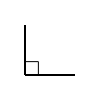
\includegraphics[scale=\shrinkfactor]{figures/e6ad77b54552295693aae7e39624ed456b552099.png}

A right triangle contains one right angle.

\paragraph{Hint 2}An acute angle is less than $90 ^\circ$.

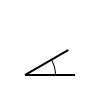
\includegraphics[scale=\shrinkfactor]{figures/d3a2a4fb2274b18d8b340c80127ae99c1ed8b1f9.png}

An acute triangle has all acute angles.

\paragraph{Hint 3}An obtuse angle is more than $90 ^\circ$.

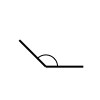
\includegraphics[scale=\shrinkfactor]{figures/3b29cb7bd47c46eb2ecd140dd305d1123b9185e6.png}

An obtuse triangle has one obtuse angle.

\paragraph{Hint 4}Right Triangles


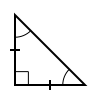
\includegraphics[scale=\shrinkfactor]{figures/8837c2c90c5edbd24cdce3fa7e110370dd5dcdef.png}


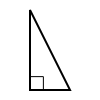
\includegraphics[scale=\shrinkfactor]{figures/ac56df552ee790942f862b76d637a69c2180f1d4.png}

Obtuse Triangles


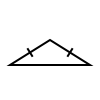
\includegraphics[scale=\shrinkfactor]{figures/ab33a8ea9f6040b7277f725f46c6d9452ab8fbbc.png}

Acute Triangles


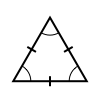
\includegraphics[scale=\shrinkfactor]{figures/2e6355867a1027528f1719f9dcb578dcb221b055.png}


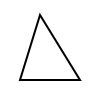
\includegraphics[scale=\shrinkfactor]{figures/ee7f87a00acb47dec4f2b2eed9a6741b21afc47d.png}



\medskip
\noindent
\textbf{Tags:} {\footnotesize CC.4.G.A.2, Properties of shapes 1, SB.4.1.L.4.TE, SB.4.1.L.4.CR, SB.4.1.L.5.TE}\\
\textbf{Version:} f508765c.. 2013-10-06
\smallskip\hrule





\section{\href{https://www.khanacademy.org/devadmin/content/items/x240f55e2c1c2b7ed}{x240f55e2c1c2b7ed}}

\noindent
**Which side is parallel to side $\overline{BC}$?**


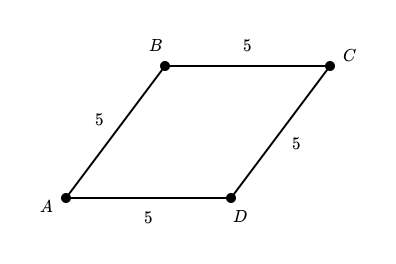
\includegraphics[scale=\shrinkfactor]{figures/84f3fcb82754c1a5d2b6c841c69a1a562675f88b.png}

\paragraph{Ans} Side [[? expression 1]] is parallel.
  AD

\paragraph{Hint 1}Parallel lines always remain the same distance apart and therefore never intersect. 

\paragraph{Hint 2}
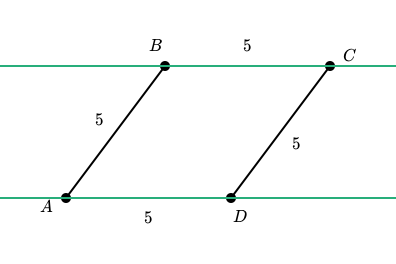
\includegraphics[scale=\shrinkfactor]{figures/677e2bdf627d0186c2d7eb494916d32d1ab4f1d0.png}

\paragraph{Hint 3}Side $\overline{AD}$ is parallel to side $\overline{BC}$.



\medskip
\noindent
\textbf{Tags:} {\footnotesize CC.4.G.A.2, Properties of shapes 1, SB.4.1.L.4.TE, SB.4.1.L.4.CR, SB.4.1.L.5.TE}\\
\textbf{Version:} f87804af.. 2013-10-10
\smallskip\hrule





\section{\href{https://www.khanacademy.org/devadmin/content/items/x24d50dbce8e569b5}{x24d50dbce8e569b5}}

\noindent
**Put the triangles into the correct categories.**
[[? categorization 1]]


\paragraph{Ans} Drag and drop each card into the appropriate category. 

\paragraph{Hint 1}A right angle is $90 ^\circ$.

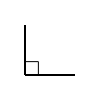
\includegraphics[scale=\shrinkfactor]{figures/e6ad77b54552295693aae7e39624ed456b552099.png}

A right triangle contains one right angle.

\paragraph{Hint 2}An acute angle is less than $90 ^\circ$.

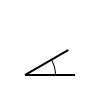
\includegraphics[scale=\shrinkfactor]{figures/d3a2a4fb2274b18d8b340c80127ae99c1ed8b1f9.png}

An acute triangle has all acute angles.

\paragraph{Hint 3}An obtuse angle is more than $90 ^\circ$.

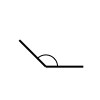
\includegraphics[scale=\shrinkfactor]{figures/3b29cb7bd47c46eb2ecd140dd305d1123b9185e6.png}

An obtuse triangle has one obtuse angle.

\paragraph{Hint 4}Right Triangles


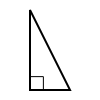
\includegraphics[scale=\shrinkfactor]{figures/ac56df552ee790942f862b76d637a69c2180f1d4.png}

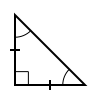
\includegraphics[scale=\shrinkfactor]{figures/8837c2c90c5edbd24cdce3fa7e110370dd5dcdef.png}

Obtuse Triangles


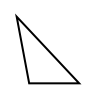
\includegraphics[scale=\shrinkfactor]{figures/2d844a51b839d81f30ea0fd7869869c78159abd0.png} 
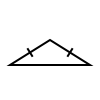
\includegraphics[scale=\shrinkfactor]{figures/ab33a8ea9f6040b7277f725f46c6d9452ab8fbbc.png}

Acute Triangles


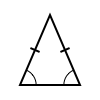
\includegraphics[scale=\shrinkfactor]{figures/dc310510e56d5d165e56b2b2a168163c503fe100.png}

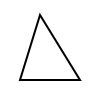
\includegraphics[scale=\shrinkfactor]{figures/ee7f87a00acb47dec4f2b2eed9a6741b21afc47d.png}



\medskip
\noindent
\textbf{Tags:} {\footnotesize CC.4.G.A.2, Properties of shapes 1, SB.4.1.L.4.TE, SB.4.1.L.4.CR, SB.4.1.L.5.TE}\\
\textbf{Version:} 1c878643.. 2013-10-15
\smallskip\hrule





\section{\href{https://www.khanacademy.org/devadmin/content/items/x2cd03f4961977251}{x2cd03f4961977251}}

\noindent
**Which side is perpendicular to side $\overline{BC}$?**

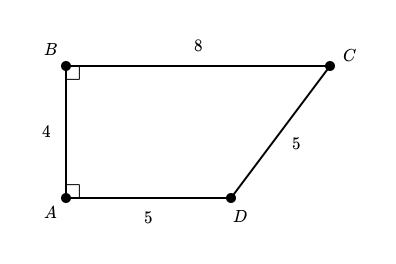
\includegraphics[scale=\shrinkfactor]{figures/af1e22d3573a0a03d6cfa63d1c97705f69e1336c.png}

\paragraph{Ans} Side  [[? expression 1]] is perpendicular.
  AB

\paragraph{Hint 1}Perpendicular lines intersect at a $90 ^\circ$ angle.  
A right angle is in the shape of a perfect corner, like the corner of a typical sheet of paper.


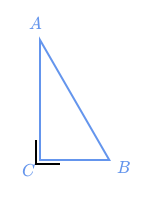
\includegraphics[scale=\shrinkfactor]{figures/497661f48f441186b5e021d8ca8c4f0c7449214f.png}

\paragraph{Hint 2}Side $\overline{BC}$ intersects with both $\overline{AB}$ and $\overline{CD}$ but is only perpendicular with one.

\paragraph{Hint 3}Side $\overline{AB}$ forms a right angle with side $\overline{BC}$.

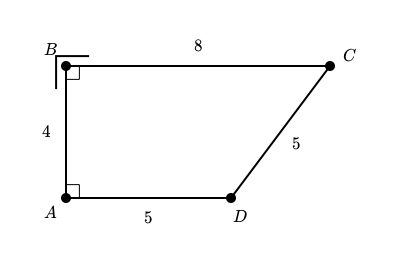
\includegraphics[scale=\shrinkfactor]{figures/88ceec57d0f6a64b4e8579ee9877e14f3e9b6889.png}



\medskip
\noindent
\textbf{Tags:} {\footnotesize CC.4.G.A.2, Properties of shapes 1, SB.4.1.L.4.TE, SB.4.1.L.4.CR, SB.4.1.L.5.TE}\\
\textbf{Version:} 4bdb1038.. 2013-10-11
\smallskip\hrule





\section{\href{https://www.khanacademy.org/devadmin/content/items/x317938291de8088a}{x317938291de8088a}}

\noindent
**Why are these shapes categorized into Group One and Group Two?**
 
Group One


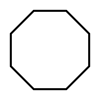
\includegraphics[scale=\shrinkfactor]{figures/7d98a99c75a84da8f748444ad7a3a8053be16a27.png}

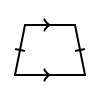
\includegraphics[scale=\shrinkfactor]{figures/f6970c7834b69ce137488d985cb48d2f38c66936.png}

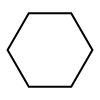
\includegraphics[scale=\shrinkfactor]{figures/0245164f3f4897772e76d361f955075a80732b03.png}

Group Two


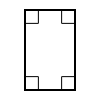
\includegraphics[scale=\shrinkfactor]{figures/de8e97f23717ff840eeffe53dee6e1dc88c119fa.png}

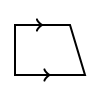
\includegraphics[scale=\shrinkfactor]{figures/53c957e1607d463070480943456fd8435ab45b5d.png}

\paragraph{Ans} 

One group has parallel lines but the other does not.

One group has only equilateral shapes and the other has only shapes that are not equilateral.

One group has shapes with four sides and the other has shapes with more than four sides.

\fbox{ One group has perpendicular lines but the other does not.

}

 

\paragraph{Hint 1}Parallel lines always remain the same distance apart and therefore never intersect.  Look at the pair of parallel lines below.  No matter how far they are extended, they will never meet.

$\phantom{xxxx}$

\includegraphics[scale=\shrinkfactor]{figures/7cf1fbfb7516a57d37ad80007a3886c81c33f393.png}  
All the shapes have parallel lines so that is not the correct answer.

\paragraph{Hint 2}Equilateral shapes have sides of equal lengths.  Only the hexagon has equal lengths so this is not the correct answer.

\paragraph{Hint 3}All these shapes have four sides except the hexagon so this is not the correct answer.

\paragraph{Hint 4}Group One

$\phantom{xxxx}$
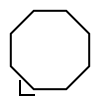
\includegraphics[scale=\shrinkfactor]{figures/e545f7ea1f54d28f35d3f53800176fa61cfa576a.png}
$\phantom{xxxx}$
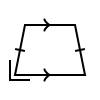
\includegraphics[scale=\shrinkfactor]{figures/0551b3aafe67b1364e8c26b46976f33448514e73.png}
$\phantom{xxxx}$
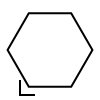
\includegraphics[scale=\shrinkfactor]{figures/86b2c3c3c0943d023a08a365d4a9966c85516b6a.png}

Group Two

$\phantom{xxxx}$
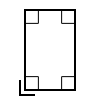
\includegraphics[scale=\shrinkfactor]{figures/d6d791274da0b0e2e00f611eecdc6fbff3b6f565.png}
$\phantom{xxxx}$
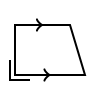
\includegraphics[scale=\shrinkfactor]{figures/b40fe0d71041d95a6048607b1a3b833ea4457558.png}

\paragraph{Hint 5}The first group has no perpendicular lines.  The second group has perpendicular lines.



\medskip
\noindent
\textbf{Tags:} {\footnotesize CC.4.G.A.2, Properties of shapes 1, SB.4.1.L.4.TE, SB.4.1.L.4.CR, SB.4.1.L.5.TE}\\
\textbf{Version:} 46c81feb.. 2013-10-11
\smallskip\hrule





\section{\href{https://www.khanacademy.org/devadmin/content/items/x323f763994b14c7b}{x323f763994b14c7b}}

\noindent
**Which side is parallel to side $\overline{AF}$?**


\includegraphics[scale=\shrinkfactor]{figures/28503190185ac259dd94d90087b4ef7971a78c3e.png}

\paragraph{Ans} Side  [[? expression 1]] is parallel.
  CD

\paragraph{Hint 1}Parallel lines always remain the same distance apart and therefore never intersect. 

\paragraph{Hint 2}
\includegraphics[scale=\shrinkfactor]{figures/0785bb6725a0a8c444685da8dcf856a59a09aacc.png}

\paragraph{Hint 3}Side $\overline{CD}$ is parallel to side $\overline{AF}$.



\medskip
\noindent
\textbf{Tags:} {\footnotesize CC.4.G.A.2, Properties of shapes 1, SB.4.1.L.4.TE, SB.4.1.L.4.CR, SB.4.1.L.5.TE}\\
\textbf{Version:} 6ad43ff6.. 2013-10-11
\smallskip\hrule





\section{\href{https://www.khanacademy.org/devadmin/content/items/x386c27c44312579f}{x386c27c44312579f}}

\noindent
**Put the shapes into the correct categories.**

[[? categorization 1]]


\paragraph{Ans} Drag and drop each card into the appropriate category. 

\paragraph{Hint 1}Parallel lines always remain the same distance apart and therefore never intersect.  Look at the pair of parallel lines below.  No matter how far they are extended, they will never meet.

$\phantom{xxxx}$
\includegraphics[scale=\shrinkfactor]{figures/7cf1fbfb7516a57d37ad80007a3886c81c33f393.png}

\paragraph{Hint 2} Perpendicular lines intersect at a $90 ^\circ$ angle.  
A right angle is in the shape of a perfect corner, like the corner of a typical sheet of paper.


\includegraphics[scale=\shrinkfactor]{figures/497661f48f441186b5e021d8ca8c4f0c7449214f.png}

\paragraph{Hint 3}Parallel lines only:

$\phantom{xxxxxxxx}$
\includegraphics[scale=\shrinkfactor]{figures/dc97e97ad57144cae5a8b5bfdc5d541d8d66aa00.png}
 
$\phantom{xxxxxxxx}$
\includegraphics[scale=\shrinkfactor]{figures/a8914ec8b688d03af4fc47bdfdb83edcce453d65.png}

Perpendicular lines only:

$\phantom{xxxxxxxx}$
\includegraphics[scale=\shrinkfactor]{figures/22dbb4135afcdee971b389f3b794eb3a9a08ea40.png}

$\phantom{xxxxxxxx}$
\includegraphics[scale=\shrinkfactor]{figures/789e2f97ce566bdea069b01d730472c5c267c9de.png}

Both parallel and perpendicular lines:

$\phantom{xxxxxxxx}$
\includegraphics[scale=\shrinkfactor]{figures/ad42bf00e54b665d02d6e9aa787d9d04875ccc6e.png}

$\phantom{xxxxxxxx}$
\includegraphics[scale=\shrinkfactor]{figures/83e816a8326a20f4b9c025cf8634a5a1a67c87ce.png}



\medskip
\noindent
\textbf{Tags:} {\footnotesize CC.4.G.A.2, Properties of shapes 1, SB.4.1.L.4.TE, SB.4.1.L.4.CR, SB.4.1.L.5.TE}\\
\textbf{Version:} 24f5b42e.. 2013-10-15
\smallskip\hrule





\section{\href{https://www.khanacademy.org/devadmin/content/items/x49625710d1bdb0ff}{x49625710d1bdb0ff}}

\noindent
**Which side is parallel to side $\overline{AB}$?**


\includegraphics[scale=\shrinkfactor]{figures/84f3fcb82754c1a5d2b6c841c69a1a562675f88b.png}

\paragraph{Ans} Side  [[? expression 1]] is parallel.
  CD

\paragraph{Hint 1}Parallel lines always remain the same distance apart and therefore never intersect. 

\paragraph{Hint 2}
\includegraphics[scale=\shrinkfactor]{figures/5171a6475c1016e0d75473bd038031d9f41676df.png}

\paragraph{Hint 3}Side $\overline{CD}$ is parallel to side $\overline{AB}$.



\medskip
\noindent
\textbf{Tags:} {\footnotesize CC.4.G.A.2, Properties of shapes 1, SB.4.1.L.4.TE, SB.4.1.L.4.CR, SB.4.1.L.5.TE}\\
\textbf{Version:} d7d66f6e.. 2013-10-11
\smallskip\hrule





\section{\href{https://www.khanacademy.org/devadmin/content/items/x574cb9df16bec506}{x574cb9df16bec506}}

\noindent
**Which side is parallel to side $\overline{AB}$?**


\includegraphics[scale=\shrinkfactor]{figures/8416b01e9ba095ab2d9c78d8fdec2e38ff55813b.png}

\paragraph{Ans} Side  [[? expression 1]] is parallel.
  DE

\paragraph{Hint 1}Parallel lines always remain the same distance apart and therefore never intersect. 

\paragraph{Hint 2}
\includegraphics[scale=\shrinkfactor]{figures/7fea3dbf376fe14f5825d4a39218b52942381530.png}

\paragraph{Hint 3}Side $\overline{DE}$ is parallel to side $\overline{AB}$.



\medskip
\noindent
\textbf{Tags:} {\footnotesize CC.4.G.A.2, Properties of shapes 1, SB.4.1.L.4.TE, SB.4.1.L.4.CR, SB.4.1.L.5.TE}\\
\textbf{Version:} 67a9337a.. 2013-10-14
\smallskip\hrule





\section{\href{https://www.khanacademy.org/devadmin/content/items/x5c9360f835aabca5}{x5c9360f835aabca5}}

\noindent
**Why are these shapes categorized into Group One and Group Two?** 

Group One 



\includegraphics[scale=\shrinkfactor]{figures/498a6b09730fdba2360826c138eeee142e8cccc1.png}

\includegraphics[scale=\shrinkfactor]{figures/d7e87a3d879924b2a1dbf230d26c2ff999761993.png}
![](https://ka-perseus-graphie.s3.amazonaws.com/2e6355867a1027528f1719f9dcb578dcb221b055.png
)

Group Two

![](https://ka-perseus-graphie.s3.amazonaws.com/2d844a51b839d81f30ea0fd7869869c78159abd0.png
 )

\includegraphics[scale=\shrinkfactor]{figures/be0b4c8e85edc438c12910c91d66875e8fcd2372.png}

\includegraphics[scale=\shrinkfactor]{figures/ee7f87a00acb47dec4f2b2eed9a6741b21afc47d.png}



\paragraph{Ans} 

One group has parallel lines but the other does not.

\fbox{ One group has only equilateral shapes and the other has only shapes that are not equilateral.

}

 One group has shapes with four sides and the other has shapes that are not four sides.

One group has perpendicular lines but the other does not.



\paragraph{Hint 1}Parallel lines always remain the same distance apart and therefore never intersect.  Look at the pair of parallel lines below.  No matter how far they are extended, they will never meet.

$\phantom{xxxx}$
\includegraphics[scale=\shrinkfactor]{figures/7cf1fbfb7516a57d37ad80007a3886c81c33f393.png}  

Both groups have shapes that have parallel lines and shapes that don't have parallel lines.

\paragraph{Hint 2}Both groups have shapes that are not four sides (both have triangles).

\paragraph{Hint 3}Perpendicular lines intersect at a $90 ^\circ$ angle.
A right angle is in the shape of a perfect corner, like the corner of a typical sheet of paper.  Only one shape in the second group has perpendicular lines.

\paragraph{Hint 4}Equilateral shapes have sides of equal lengths.  The sides of the hexagon, the pentagon and the triangle are each equal.

\paragraph{Hint 5}The first group has only equilateral shapes and the second group has only shapes that are not equilateral.



\medskip
\noindent
\textbf{Tags:} {\footnotesize CC.4.G.A.2, Properties of shapes 1, SB.4.1.L.4.TE, SB.4.1.L.4.CR, SB.4.1.L.5.TE}\\
\textbf{Version:} 2928cd1f.. 2013-10-14
\smallskip\hrule





\section{\href{https://www.khanacademy.org/devadmin/content/items/x6cc61a983d665dfd}{x6cc61a983d665dfd}}

\noindent
**Which two sides are perpendicular?**


\includegraphics[scale=\shrinkfactor]{figures/e89694af7de05350f951069a187e20d95da00947.png}

\paragraph{Ans} Side  [[? expression 1]] and Side  [[? expression 2]] are perpendicular.  CD

\paragraph{Hint 1}Perpendicular lines intersect at a $90 ^\circ$ angle.  
A right angle is in the shape of a perfect corner, like the corner of a typical sheet of paper.


\includegraphics[scale=\shrinkfactor]{figures/497661f48f441186b5e021d8ca8c4f0c7449214f.png}

\paragraph{Hint 2}Side $\overline{DE}$ forms a right angle with side $\overline{CD}$.

\includegraphics[scale=\shrinkfactor]{figures/6c13c7c1fe841eb9f59f05098c59c6e31e785bcb.png}



\medskip
\noindent
\textbf{Tags:} {\footnotesize CC.4.G.A.2, Properties of shapes 1, SB.4.1.L.4.TE, SB.4.1.L.4.CR, SB.4.1.L.5.TE}\\
\textbf{Version:} 0e0a750a.. 2013-10-14
\smallskip\hrule





\section{\href{https://www.khanacademy.org/devadmin/content/items/x86ed4058d37b653d}{x86ed4058d37b653d}}

\noindent
**Why are these shapes categorized into Group One and Group Two?** 

Group One 


\includegraphics[scale=\shrinkfactor]{figures/feaa75a1e077e1d8ea6873bc2a4aa206d3c95598.png} 
\includegraphics[scale=\shrinkfactor]{figures/53c957e1607d463070480943456fd8435ab45b5d.png} 
\includegraphics[scale=\shrinkfactor]{figures/be0b4c8e85edc438c12910c91d66875e8fcd2372.png}

Group Two


\includegraphics[scale=\shrinkfactor]{figures/0245164f3f4897772e76d361f955075a80732b03.png} 
\includegraphics[scale=\shrinkfactor]{figures/ee7f87a00acb47dec4f2b2eed9a6741b21afc47d.png} 
\includegraphics[scale=\shrinkfactor]{figures/498a6b09730fdba2360826c138eeee142e8cccc1.png}


\paragraph{Ans} 

One group has parallel lines but the other does not.

One group has only equilateral shapes and the other has only shapes that are not equilateral.

\fbox{ One group only has quadrilaterals and the other does not.

}

 One group has perpendicular lines but the other does not.



\paragraph{Hint 1}Parallel lines always remain the same distance apart and therefore never intersect.  Look at the pair of parallel lines below.  No matter how far they are extended, they will never meet.

$\phantom{xxxx}$
\includegraphics[scale=\shrinkfactor]{figures/7cf1fbfb7516a57d37ad80007a3886c81c33f393.png}  

Both groups have parallel lines.  Look at the first one in each group.

\paragraph{Hint 2}Equilateral shapes have sides of equal lengths.  Only the hexagon and the pentagon have equal lengths so this is not the correct answer.

\paragraph{Hint 3}Perpendicular lines intersect at a $90 ^\circ$ angle.
A right angle is in the shape of a perfect corner, like the corner of a typical sheet of paper.  None of the shapes has perpendicular lines.

\paragraph{Hint 4}Quadrilaterals are shapes with four sides.  All the figures in Group One have four sides.  None of the shapes in Group Two have four sides.



\medskip
\noindent
\textbf{Tags:} {\footnotesize CC.4.G.A.2, Properties of shapes 1, SB.4.1.L.4.TE, SB.4.1.L.4.CR, SB.4.1.L.5.TE}\\
\textbf{Version:} 6b2fce4e.. 2013-10-12
\smallskip\hrule





\section{\href{https://www.khanacademy.org/devadmin/content/items/x8e61ce25750fc85a}{x8e61ce25750fc85a}}

\noindent
**Which side is perpendicular to side $\overline{CD}$?**


\includegraphics[scale=\shrinkfactor]{figures/e89694af7de05350f951069a187e20d95da00947.png}

\paragraph{Ans} Side  [[? expression 1]] is perpendicular.
  DE

\paragraph{Hint 1}Perpendicular lines intersect at a $90 ^\circ$ angle.  
A right angle is in the shape of a perfect corner, like the corner of a typical sheet of paper.


\includegraphics[scale=\shrinkfactor]{figures/497661f48f441186b5e021d8ca8c4f0c7449214f.png}

\paragraph{Hint 2}Side $\overline{CD}$ intersects with both $\overline{BC}$ and $\overline{DE}$ but is only perpendicular with one.

\paragraph{Hint 3}Side $\overline{DE}$ forms a right angle with side $\overline{CD}$.

\includegraphics[scale=\shrinkfactor]{figures/6c13c7c1fe841eb9f59f05098c59c6e31e785bcb.png}



\medskip
\noindent
\textbf{Tags:} {\footnotesize CC.4.G.A.2, Properties of shapes 1, SB.4.1.L.4.TE, SB.4.1.L.4.CR, SB.4.1.L.5.TE}\\
\textbf{Version:} 31fa242c.. 2013-10-14
\smallskip\hrule





\section{\href{https://www.khanacademy.org/devadmin/content/items/xa164f0a66db8a4a5}{xa164f0a66db8a4a5}}

\noindent
**Which side is parallel to side $\overline{BC}$?**


\includegraphics[scale=\shrinkfactor]{figures/e89694af7de05350f951069a187e20d95da00947.png}

\paragraph{Ans} Side  [[? expression 1]] is perpendicular.
  AE

\paragraph{Hint 1}Parallel lines always remain the same distance apart and therefore never intersect. 

\paragraph{Hint 2}
\includegraphics[scale=\shrinkfactor]{figures/8037be89852b1d59afbf6ea45e9d72c8640c7e6b.png}

\paragraph{Hint 3}Side $\overline{AE}$ is parallel to side $\overline{BC}$.



\medskip
\noindent
\textbf{Tags:} {\footnotesize CC.4.G.A.2, Properties of shapes 1, SB.4.1.L.4.TE, SB.4.1.L.4.CR, SB.4.1.L.5.TE}\\
\textbf{Version:} c5195e2f.. 2013-10-14
\smallskip\hrule





\section{\href{https://www.khanacademy.org/devadmin/content/items/xa53b2125b79013ea}{xa53b2125b79013ea}}

\noindent
**Which side is perpendicular to side $\overline{AB}$?**

\includegraphics[scale=\shrinkfactor]{figures/bfb555fa03fa87c5686e4050e123efb878484344.png}

\paragraph{Ans} Side  [[? expression 1]] is perpendicular.
  AE

\paragraph{Hint 1}Perpendicular lines intersect at a $90 ^\circ$ angle.  
A right angle is in the shape of a perfect corner, like the corner of a typical sheet of paper.


\includegraphics[scale=\shrinkfactor]{figures/497661f48f441186b5e021d8ca8c4f0c7449214f.png}

\paragraph{Hint 2}Side $\overline{AB}$ intersects with both $\overline{BC}$ and $\overline{AE}$ but is only perpendicular with one.

\paragraph{Hint 3}Side $\overline{AB}$ forms a right angle with side $\overline{AE}$.

\includegraphics[scale=\shrinkfactor]{figures/ac2de68945d2c7eea7f72f353d3f700df291dd2d.png}



\medskip
\noindent
\textbf{Tags:} {\footnotesize CC.4.G.A.2, Properties of shapes 1, SB.4.1.L.4.TE, SB.4.1.L.4.CR, SB.4.1.L.5.TE}\\
\textbf{Version:} 9b9ac112.. 2013-10-11
\smallskip\hrule





\section{\href{https://www.khanacademy.org/devadmin/content/items/xab814c0bdd23ef28}{xab814c0bdd23ef28}}

\noindent
**Put the triangles into the correct categories.**
[[? categorization 1]]


\paragraph{Ans} Drag and drop each card into the appropriate category. 

\paragraph{Hint 1}A equilateral triangle has three equal sides.



\paragraph{Hint 2}An isosceles triangle has two equal sides.

\paragraph{Hint 3}A scalene triangle has no equal sides.

\paragraph{Hint 4}Scalene Triangles


\includegraphics[scale=\shrinkfactor]{figures/ee7f87a00acb47dec4f2b2eed9a6741b21afc47d.png}


\includegraphics[scale=\shrinkfactor]{figures/ac56df552ee790942f862b76d637a69c2180f1d4.png}

Isosceles Triangles


\includegraphics[scale=\shrinkfactor]{figures/dc310510e56d5d165e56b2b2a168163c503fe100.png}


\includegraphics[scale=\shrinkfactor]{figures/ab33a8ea9f6040b7277f725f46c6d9452ab8fbbc.png}

Equilateral Triangles


\includegraphics[scale=\shrinkfactor]{figures/2e6355867a1027528f1719f9dcb578dcb221b055.png}



\medskip
\noindent
\textbf{Tags:} {\footnotesize CC.4.G.A.2, Properties of shapes 1, SB.4.1.L.4.TE, SB.4.1.L.4.CR, SB.4.1.L.5.TE}\\
\textbf{Version:} 5d5cd341.. 2013-10-06
\smallskip\hrule





\section{\href{https://www.khanacademy.org/devadmin/content/items/xabc13ac997f943bd}{xabc13ac997f943bd}}

\noindent
**Put the shapes into the correct categories.**

[[? categorization 1]]


\paragraph{Ans} Drag and drop each card into the appropriate category. 

\paragraph{Hint 1}Parallel lines always remain the same distance apart and therefore never intersect.  Look at the pair of parallel lines below.  No matter how far they are extended, they will never meet.

$\phantom{xxxx}$
\includegraphics[scale=\shrinkfactor]{figures/7cf1fbfb7516a57d37ad80007a3886c81c33f393.png}

\paragraph{Hint 2} Perpendicular lines intersect at a $90 ^\circ$ angle.  
A right angle is in the shape of a perfect corner, like the corner of a typical sheet of paper.


\includegraphics[scale=\shrinkfactor]{figures/497661f48f441186b5e021d8ca8c4f0c7449214f.png}

\paragraph{Hint 3}Parallel lines only:

$\phantom{xxxxxxxx}$
\includegraphics[scale=\shrinkfactor]{figures/dc97e97ad57144cae5a8b5bfdc5d541d8d66aa00.png}
 
$\phantom{xxxxxxxx}$
\includegraphics[scale=\shrinkfactor]{figures/a8914ec8b688d03af4fc47bdfdb83edcce453d65.png}

Perpendicular lines only:

$\phantom{xxxxxxxx}$
\includegraphics[scale=\shrinkfactor]{figures/f9413d967bb68c6b85d95672324c0a5b08af982e.png}

$\phantom{xxxxxxxx}$
\includegraphics[scale=\shrinkfactor]{figures/789e2f97ce566bdea069b01d730472c5c267c9de.png}

Both parallel and perpendicular lines:

$\phantom{xxxxxxxx}$
\includegraphics[scale=\shrinkfactor]{figures/ad42bf00e54b665d02d6e9aa787d9d04875ccc6e.png}

$\phantom{xxxxxxxx}$
\includegraphics[scale=\shrinkfactor]{figures/c755ceca3f49cc6303844bb5cd33f40647ddfab0.png}



\medskip
\noindent
\textbf{Tags:} {\footnotesize CC.4.G.A.2, Properties of shapes 1, SB.4.1.L.4.TE, SB.4.1.L.4.CR, SB.4.1.L.5.TE}\\
\textbf{Version:} e62ccf3c.. 2013-10-11
\smallskip\hrule





\section{\href{https://www.khanacademy.org/devadmin/content/items/xb8690ef368189333}{xb8690ef368189333}}

\noindent
**Which side is perpendicular to side $\overline{AD}$?**

\includegraphics[scale=\shrinkfactor]{figures/af1e22d3573a0a03d6cfa63d1c97705f69e1336c.png}

\paragraph{Ans} Side  [[? expression 1]] is perpendicular.
  AB

\paragraph{Hint 1}Perpendicular lines intersect at a $90 ^\circ$ angle.  
A right angle is in the shape of a perfect corner, like the corner of a typical sheet of paper.


\includegraphics[scale=\shrinkfactor]{figures/497661f48f441186b5e021d8ca8c4f0c7449214f.png}

\paragraph{Hint 2}Side $\overline{AD}$ intersects with both $\overline{AB}$ and $\overline{CD}$ but is only perpendicular with one.

\paragraph{Hint 3}Side $\overline{AB}$ forms a right angle with side $\overline{AD}$.

\includegraphics[scale=\shrinkfactor]{figures/9b7dfefa037b648abfb4816b1dff8de898e30b36.png}



\medskip
\noindent
\textbf{Tags:} {\footnotesize CC.4.G.A.2, Properties of shapes 1, SB.4.1.L.4.TE, SB.4.1.L.4.CR, SB.4.1.L.5.TE}\\
\textbf{Version:} 8aff8d84.. 2013-10-14
\smallskip\hrule





\section{\href{https://www.khanacademy.org/devadmin/content/items/xc91364af69a929a0}{xc91364af69a929a0}}

\noindent
**Which side is perpendicular to side $\overline{DE}$?**

\includegraphics[scale=\shrinkfactor]{figures/3a5627b228409ceef6d5626dd0a440d65e019442.png}

\paragraph{Ans} Side  [[? expression 1]] is perpendicular.
  CD

\paragraph{Hint 1}Perpendicular lines intersect at a $90 ^\circ$ angle.  
A right angle is in the shape of a perfect corner, like the corner of a typical sheet of paper.


\includegraphics[scale=\shrinkfactor]{figures/497661f48f441186b5e021d8ca8c4f0c7449214f.png}

\paragraph{Hint 2}Side $\overline{DE}$ intersects with both $\overline{CD}$ and $\overline{AE}$ but is only perpendicular with one.

\paragraph{Hint 3}Side $\overline{CD}$ forms a right angle with side $\overline{DE}$.

\includegraphics[scale=\shrinkfactor]{figures/e2ebf7a945c31e610b7b3bc519435119ab626207.png}



\medskip
\noindent
\textbf{Tags:} {\footnotesize CC.4.G.A.2, Properties of shapes 1, SB.4.1.L.4.TE, SB.4.1.L.4.CR, SB.4.1.L.5.TE}\\
\textbf{Version:} c2801d08.. 2013-10-14
\smallskip\hrule





\section{\href{https://www.khanacademy.org/devadmin/content/items/xc9a08e438dc1e20f}{xc9a08e438dc1e20f}}

\noindent
**Why are these shapes categorized into Group One and Group Two?** 

Group One 


\includegraphics[scale=\shrinkfactor]{figures/feaa75a1e077e1d8ea6873bc2a4aa206d3c95598.png}

\includegraphics[scale=\shrinkfactor]{figures/0245164f3f4897772e76d361f955075a80732b03.png}

\includegraphics[scale=\shrinkfactor]{figures/53c957e1607d463070480943456fd8435ab45b5d.png}


Group Two


\includegraphics[scale=\shrinkfactor]{figures/be0b4c8e85edc438c12910c91d66875e8fcd2372.png}

\includegraphics[scale=\shrinkfactor]{figures/ee7f87a00acb47dec4f2b2eed9a6741b21afc47d.png}

\includegraphics[scale=\shrinkfactor]{figures/498a6b09730fdba2360826c138eeee142e8cccc1.png}


\paragraph{Ans} 

\fbox{ One group has parallel lines but the other does not.

}

 One group has only equilateral shapes and the other has only shapes that are not equilateral.

One group has shapes with four sides and the other has shapes that are not four sides.

One group has perpendicular lines but the other does not.



\paragraph{Hint 1}Equilateral shapes have sides of equal lengths.  Only the hexagon and the pentagon have equal lengths so this is not the correct answer.

\paragraph{Hint 2}Both groups have shapes with more than four sides.  The second group also has has shapes with three sides.

\paragraph{Hint 3}Perpendicular lines intersect at a $90 ^\circ$ angle.
A right angle is in the shape of a perfect corner, like the corner of a typical sheet of paper.  None of the shapes has perpendicular lines.

\paragraph{Hint 4}Parallel lines always remain the same distance apart and therefore never intersect.  Look at the pair of parallel lines below.  No matter how far they are extended, they will never meet.

$\phantom{xxxx}$
\includegraphics[scale=\shrinkfactor]{figures/7cf1fbfb7516a57d37ad80007a3886c81c33f393.png}  


\paragraph{Hint 5}Group One 


\includegraphics[scale=\shrinkfactor]{figures/dc97e97ad57144cae5a8b5bfdc5d541d8d66aa00.png}$\phantom{xxx}$
\includegraphics[scale=\shrinkfactor]{figures/a8914ec8b688d03af4fc47bdfdb83edcce453d65.png}$\phantom{xxx}$
\includegraphics[scale=\shrinkfactor]{figures/c65c46cb76be1527eb7ded9b879ae1272452b7a1.png}  


Group Two


\includegraphics[scale=\shrinkfactor]{figures/2d844a51b839d81f30ea0fd7869869c78159abd0.png}

\includegraphics[scale=\shrinkfactor]{figures/ee7f87a00acb47dec4f2b2eed9a6741b21afc47d.png}

\includegraphics[scale=\shrinkfactor]{figures/498a6b09730fdba2360826c138eeee142e8cccc1.png}


\paragraph{Hint 6}The first group has parallel lines.  The second group has no parallel lines.



\medskip
\noindent
\textbf{Tags:} {\footnotesize CC.4.G.A.2, Properties of shapes 1, SB.4.1.L.4.TE, SB.4.1.L.4.CR, SB.4.1.L.5.TE}\\
\textbf{Version:} 1e9d45e5.. 2013-10-12
\smallskip\hrule





\section{\href{https://www.khanacademy.org/devadmin/content/items/xd6759940d63f0ecd}{xd6759940d63f0ecd}}

\noindent
**Put the shapes into the correct categories.**

[[? categorization 1]]


\paragraph{Ans} Drag and drop each card into the appropriate category. 

\paragraph{Hint 1}Parallel lines always remain the same distance apart and therefore never intersect.  Look at the pair of parallel lines below.  No matter how far they are extended, they will never meet.

$\phantom{xxxx}$
\includegraphics[scale=\shrinkfactor]{figures/7cf1fbfb7516a57d37ad80007a3886c81c33f393.png}

\paragraph{Hint 2} Perpendicular lines intersect at a $90 ^\circ$ angle.  
A right angle is in the shape of a perfect corner, like the corner of a typical sheet of paper.


\includegraphics[scale=\shrinkfactor]{figures/497661f48f441186b5e021d8ca8c4f0c7449214f.png}

\paragraph{Hint 3}Parallel lines only:

$\phantom{xxxxxxxx}$
\includegraphics[scale=\shrinkfactor]{figures/dc97e97ad57144cae5a8b5bfdc5d541d8d66aa00.png}

\includegraphics[scale=\shrinkfactor]{figures/68da9c12f9a5652bcfd03be81ae13785412b510b.png}  
$\phantom{xxxxxxxx}$
\includegraphics[scale=\shrinkfactor]{figures/a8914ec8b688d03af4fc47bdfdb83edcce453d65.png}

Perpendicular lines only:

$\phantom{xxxxxxxx}$
\includegraphics[scale=\shrinkfactor]{figures/f9413d967bb68c6b85d95672324c0a5b08af982e.png}

Both parallel and perpendicular lines:

$\phantom{xxxxxxxx}$
\includegraphics[scale=\shrinkfactor]{figures/ad42bf00e54b665d02d6e9aa787d9d04875ccc6e.png}

$\phantom{xxxxxxxx}$
\includegraphics[scale=\shrinkfactor]{figures/c755ceca3f49cc6303844bb5cd33f40647ddfab0.png}



\medskip
\noindent
\textbf{Tags:} {\footnotesize CC.4.G.A.2, Properties of shapes 1, SB.4.1.L.4.TE, SB.4.1.L.4.CR, SB.4.1.L.5.TE}\\
\textbf{Version:} 4fd2192f.. 2013-10-04
\smallskip\hrule





\section{\href{https://www.khanacademy.org/devadmin/content/items/xd7aab48ce7221955}{xd7aab48ce7221955}}

\noindent
**Why are these shapes categorized into Group One and Group Two?**

Group One 


\includegraphics[scale=\shrinkfactor]{figures/feaa75a1e077e1d8ea6873bc2a4aa206d3c95598.png}

\includegraphics[scale=\shrinkfactor]{figures/f6970c7834b69ce137488d985cb48d2f38c66936.png}

\includegraphics[scale=\shrinkfactor]{figures/0245164f3f4897772e76d361f955075a80732b03.png}

Group Two


\includegraphics[scale=\shrinkfactor]{figures/de8e97f23717ff840eeffe53dee6e1dc88c119fa.png}

\includegraphics[scale=\shrinkfactor]{figures/53c957e1607d463070480943456fd8435ab45b5d.png}

\paragraph{Ans} 

One group has parallel lines but the other does not.

One group has only equilateral shapes and the other has only shapes that are not equilateral.

One group has shapes with four sides and the other has shapes with more than four sides.

\fbox{ One group has perpendicular lines but the other does not.

}

 

\paragraph{Hint 1}Parallel lines always remain the same distance apart and therefore never intersect.  Look at the pair of parallel lines below.  No matter how far they are extended, they will never meet.

$\phantom{xxxx}$
\includegraphics[scale=\shrinkfactor]{figures/7cf1fbfb7516a57d37ad80007a3886c81c33f393.png}  
All the shapes have parallel lines so that is not the correct answer.

\paragraph{Hint 2}Equilateral shapes have sides of equal lengths.  Only the hexagon has equal lengths so this is not the correct answer.

\paragraph{Hint 3}All these shapes have four sides except the hexagon so this is not the correct answer.

\paragraph{Hint 4}Group One

$\phantom{xxxx}$
\includegraphics[scale=\shrinkfactor]{figures/fee7e4994ef0d10862a0f686587d8d2ba79bb13e.png}
$\phantom{xxxx}$
\includegraphics[scale=\shrinkfactor]{figures/0551b3aafe67b1364e8c26b46976f33448514e73.png}
$\phantom{xxxx}$
\includegraphics[scale=\shrinkfactor]{figures/86b2c3c3c0943d023a08a365d4a9966c85516b6a.png}

Group Two

$\phantom{xxxx}$
\includegraphics[scale=\shrinkfactor]{figures/d6d791274da0b0e2e00f611eecdc6fbff3b6f565.png}
$\phantom{xxxx}$
\includegraphics[scale=\shrinkfactor]{figures/b40fe0d71041d95a6048607b1a3b833ea4457558.png}

\paragraph{Hint 5}The first group has no perpendicular lines.  The second group has perpendicular lines.



\medskip
\noindent
\textbf{Tags:} {\footnotesize CC.4.G.A.2, Properties of shapes 1, SB.4.1.L.4.TE, SB.4.1.L.4.CR, SB.4.1.L.5.TE}\\
\textbf{Version:} 78023266.. 2013-10-11
\smallskip\hrule





\section{\href{https://www.khanacademy.org/devadmin/content/items/xe67c4298cc39f407}{xe67c4298cc39f407}}

\noindent
**Why are these shapes categorized into Group One and Group Two?** 

Group One 

 
\includegraphics[scale=\shrinkfactor]{figures/53c957e1607d463070480943456fd8435ab45b5d.png} 
\includegraphics[scale=\shrinkfactor]{figures/be0b4c8e85edc438c12910c91d66875e8fcd2372.png}

\includegraphics[scale=\shrinkfactor]{figures/5b842c6adbdf4de4dba70296479b1954a2362785.png}

Group Two


\includegraphics[scale=\shrinkfactor]{figures/9bf34a29bc62816f07057d9e571de844df484cd9.png} 
\includegraphics[scale=\shrinkfactor]{figures/ee7f87a00acb47dec4f2b2eed9a6741b21afc47d.png} ![](https://ka-perseus-graphie.s3.amazonaws.com/7d98a99c75a84da8f748444ad7a3a8053be16a27.png
)


\paragraph{Ans} 

One group has parallel lines but the other does not.

One group has only equilateral shapes and the other has only shapes that are not equilateral.

\fbox{ One group only has quadrilaterals and the other does not.

}

 One group has perpendicular lines but the other does not.



\paragraph{Hint 1}Parallel lines always remain the same distance apart and therefore never intersect.  Look at the pair of parallel lines below.  No matter how far they are extended, they will never meet.

$\phantom{xxxx}$
\includegraphics[scale=\shrinkfactor]{figures/7cf1fbfb7516a57d37ad80007a3886c81c33f393.png}  

Both groups have parallel lines.  Look at the first one in each group.

\paragraph{Hint 2}Equilateral shapes have sides of equal lengths.  Only the octagon and the rhombus have equal lengths so this is not the correct answer.

\paragraph{Hint 3}Perpendicular lines intersect at a $90 ^\circ$ angle.
A right angle is in the shape of a perfect corner, like the corner of a typical sheet of paper.  Only one shape in Group One has perpendicular lines.

\paragraph{Hint 4}Quadrilaterals are shapes with four sides.  All the figures in Group One have four sides.  None of the shapes in Group Two have four sides.



\medskip
\noindent
\textbf{Tags:} {\footnotesize CC.4.G.A.2, Properties of shapes 1, SB.4.1.L.4.TE, SB.4.1.L.4.CR, SB.4.1.L.5.TE}\\
\textbf{Version:} b835a88e.. 2013-10-14
\smallskip\hrule





\section{\href{https://www.khanacademy.org/devadmin/content/items/xef94dccb618e0151}{xef94dccb618e0151}}

\noindent
**Which two sides are parallel?**


\includegraphics[scale=\shrinkfactor]{figures/0b1f52e2d56a98d5ec5f552c02f22f067ec40078.png}

\paragraph{Ans} Side  [[? expression 1]] and Side  [[? expression 2]] are parallel.  BC

\paragraph{Hint 1}Parallel lines always remain the same distance apart and therefore never intersect. 

\paragraph{Hint 2}
\includegraphics[scale=\shrinkfactor]{figures/83c724a031b6ec05f29446ad771043b503b36466.png}

\paragraph{Hint 3}Side $\overline{BC}$ is parallel to side $\overline{AE}$.



\medskip
\noindent
\textbf{Tags:} {\footnotesize CC.4.G.A.2, Properties of shapes 1, SB.4.1.L.4.TE, SB.4.1.L.4.CR, SB.4.1.L.5.TE}\\
\textbf{Version:} 7dbd9950.. 2013-10-14
\smallskip\hrule





\section{\href{https://www.khanacademy.org/devadmin/content/items/xf07d3863079a2fa0}{xf07d3863079a2fa0}}

\noindent
**Put the triangles into the correct categories.**
[[? categorization 1]]


\paragraph{Ans} Drag and drop each card into the appropriate category. 

\paragraph{Hint 1}A equilateral triangle has three equal sides.



\paragraph{Hint 2}An isosceles triangle has two equal sides.

\paragraph{Hint 3}A scalene triangle has no equal sides.

\paragraph{Hint 4}Scalene Triangles


\includegraphics[scale=\shrinkfactor]{figures/ee7f87a00acb47dec4f2b2eed9a6741b21afc47d.png}


\includegraphics[scale=\shrinkfactor]{figures/3b6a413f170d28d15c5ddce4ea5150108fc79f24.png}

Isosceles Triangles


\includegraphics[scale=\shrinkfactor]{figures/8837c2c90c5edbd24cdce3fa7e110370dd5dcdef.png}


\includegraphics[scale=\shrinkfactor]{figures/ab33a8ea9f6040b7277f725f46c6d9452ab8fbbc.png}

Equilateral Triangles


\includegraphics[scale=\shrinkfactor]{figures/2e6355867a1027528f1719f9dcb578dcb221b055.png}



\medskip
\noindent
\textbf{Tags:} {\footnotesize CC.4.G.A.2, Properties of shapes 1, SB.4.1.L.4.TE, SB.4.1.L.4.CR, SB.4.1.L.5.TE}\\
\textbf{Version:} 485b3409.. 2013-10-14
\smallskip\hrule





\section{\href{https://www.khanacademy.org/devadmin/content/items/xf2f379906493699d}{xf2f379906493699d}}

\noindent
**Put the triangles into the correct categories.**
[[? categorization 1]]


\paragraph{Ans} Drag and drop each card into the appropriate category. 

\paragraph{Hint 1}A right angle is $90 ^\circ$.

\includegraphics[scale=\shrinkfactor]{figures/e6ad77b54552295693aae7e39624ed456b552099.png}

A right triangle contains one right angle.

\paragraph{Hint 2}An acute angle is less than $90 ^\circ$.

\includegraphics[scale=\shrinkfactor]{figures/d3a2a4fb2274b18d8b340c80127ae99c1ed8b1f9.png}

An acute triangle has all acute angles.

\paragraph{Hint 3}An obtuse angle is more than $90 ^\circ$.

\includegraphics[scale=\shrinkfactor]{figures/3b29cb7bd47c46eb2ecd140dd305d1123b9185e6.png}

An obtuse triangle has one obtuse angle.

\paragraph{Hint 4}Right Triangles


\includegraphics[scale=\shrinkfactor]{figures/8837c2c90c5edbd24cdce3fa7e110370dd5dcdef.png}

\includegraphics[scale=\shrinkfactor]{figures/ac56df552ee790942f862b76d637a69c2180f1d4.png}

Obtuse Triangles


\includegraphics[scale=\shrinkfactor]{figures/ab33a8ea9f6040b7277f725f46c6d9452ab8fbbc.png} 
\includegraphics[scale=\shrinkfactor]{figures/2d844a51b839d81f30ea0fd7869869c78159abd0.png}

Acute Triangles


\includegraphics[scale=\shrinkfactor]{figures/dc310510e56d5d165e56b2b2a168163c503fe100.png}

\includegraphics[scale=\shrinkfactor]{figures/ee7f87a00acb47dec4f2b2eed9a6741b21afc47d.png}



\medskip
\noindent
\textbf{Tags:} {\footnotesize CC.4.G.A.2, Properties of shapes 1, SB.4.1.L.4.TE, SB.4.1.L.4.CR, SB.4.1.L.5.TE}\\
\textbf{Version:} d9a623d7.. 2013-10-14
\smallskip\hrule





\section{\href{https://www.khanacademy.org/devadmin/content/items/xf48f7c83eae36508}{xf48f7c83eae36508}}

\noindent
**Why are these shapes categorized into Group One and Group Two?**

Group One 


\includegraphics[scale=\shrinkfactor]{figures/feaa75a1e077e1d8ea6873bc2a4aa206d3c95598.png}

\includegraphics[scale=\shrinkfactor]{figures/0245164f3f4897772e76d361f955075a80732b03.png}
![](https://ka-perseus-graphie.s3.amazonaws.com/7d98a99c75a84da8f748444ad7a3a8053be16a27.png
)


Group Two


\includegraphics[scale=\shrinkfactor]{figures/2d844a51b839d81f30ea0fd7869869c78159abd0.png}

\includegraphics[scale=\shrinkfactor]{figures/ee7f87a00acb47dec4f2b2eed9a6741b21afc47d.png}

\includegraphics[scale=\shrinkfactor]{figures/498a6b09730fdba2360826c138eeee142e8cccc1.png}



\paragraph{Ans} 

\fbox{ One group has parallel lines but the other does not.

}

 One group has only equilateral shapes and the other has only shapes that are not equilateral.

One group has shapes with four sides and the other has shapes that are not four sides.

One group has perpendicular lines but the other does not.



\paragraph{Hint 1}Equilateral shapes have sides of equal lengths.  Only the hexagon and the pentagon have equal lengths so this is not the correct answer.

\paragraph{Hint 2}Both groups have shapes with more than four sides.  The second group also has has shapes with three sides.

\paragraph{Hint 3}Perpendicular lines intersect at a $90 ^\circ$ angle.
A right angle is in the shape of a perfect corner, like the corner of a typical sheet of paper.  None of the shapes has perpendicular lines.

\paragraph{Hint 4}Parallel lines always remain the same distance apart and therefore never intersect.  Look at the pair of parallel lines below.  No matter how far they are extended, they will never meet.

$\phantom{xxxx}$
\includegraphics[scale=\shrinkfactor]{figures/7cf1fbfb7516a57d37ad80007a3886c81c33f393.png}  


\paragraph{Hint 5}Group One 

$\phantom{xxxxxxxx}$
\includegraphics[scale=\shrinkfactor]{figures/dc97e97ad57144cae5a8b5bfdc5d541d8d66aa00.png}

\includegraphics[scale=\shrinkfactor]{figures/f73cb50d59bdab17965cbcf6a6832a26002948cb.png}  
$\phantom{xxxxxxxx}$
\includegraphics[scale=\shrinkfactor]{figures/a8914ec8b688d03af4fc47bdfdb83edcce453d65.png}

Group Two


\includegraphics[scale=\shrinkfactor]{figures/2d844a51b839d81f30ea0fd7869869c78159abd0.png}

\includegraphics[scale=\shrinkfactor]{figures/ee7f87a00acb47dec4f2b2eed9a6741b21afc47d.png}

\includegraphics[scale=\shrinkfactor]{figures/498a6b09730fdba2360826c138eeee142e8cccc1.png}


\paragraph{Hint 6}The first group has parallel lines.  The second group has no parallel lines.



\medskip
\noindent
\textbf{Tags:} {\footnotesize CC.4.G.A.2, Properties of shapes 1, SB.4.1.L.4.TE, SB.4.1.L.4.CR, SB.4.1.L.5.TE}\\
\textbf{Version:} 4742db58.. 2013-10-11
\smallskip\hrule



%%  Create a directory called 'figures' in latex dir and run the following command 
%  wget -N \
%    https://ka-perseus-graphie.s3.amazonaws.com/0b1f52e2d56a98d5ec5f552c02f22f067ec40078.png \
%    https://ka-perseus-graphie.s3.amazonaws.com/83c724a031b6ec05f29446ad771043b503b36466.png \
%    https://ka-perseus-graphie.s3.amazonaws.com/498a6b09730fdba2360826c138eeee142e8cccc1.png \
%    https://ka-perseus-graphie.s3.amazonaws.com/0245164f3f4897772e76d361f955075a80732b03.png \
%    https://ka-perseus-graphie.s3.amazonaws.com/feaa75a1e077e1d8ea6873bc2a4aa206d3c95598.png  \
%    https://ka-perseus-graphie.s3.amazonaws.com/be0b4c8e85edc438c12910c91d66875e8fcd2372.png \
%    https://ka-perseus-graphie.s3.amazonaws.com/ee7f87a00acb47dec4f2b2eed9a6741b21afc47d.png \
%    https://ka-perseus-graphie.s3.amazonaws.com/7cf1fbfb7516a57d37ad80007a3886c81c33f393.png \
%    https://ka-perseus-graphie.s3.amazonaws.com/497661f48f441186b5e021d8ca8c4f0c7449214f.png \
%    https://ka-perseus-graphie.s3.amazonaws.com/dc97e97ad57144cae5a8b5bfdc5d541d8d66aa00.png \
%    https://ka-perseus-graphie.s3.amazonaws.com/f73cb50d59bdab17965cbcf6a6832a26002948cb.png \
%    https://ka-perseus-graphie.s3.amazonaws.com/a8914ec8b688d03af4fc47bdfdb83edcce453d65.png \
%    https://ka-perseus-graphie.s3.amazonaws.com/f9413d967bb68c6b85d95672324c0a5b08af982e.png \
%    https://ka-perseus-graphie.s3.amazonaws.com/ad42bf00e54b665d02d6e9aa787d9d04875ccc6e.png \
%    https://ka-perseus-graphie.s3.amazonaws.com/c755ceca3f49cc6303844bb5cd33f40647ddfab0.png \
%    https://ka-perseus-graphie.s3.amazonaws.com/e6ad77b54552295693aae7e39624ed456b552099.png \
%    https://ka-perseus-graphie.s3.amazonaws.com/d3a2a4fb2274b18d8b340c80127ae99c1ed8b1f9.png \
%    https://ka-perseus-graphie.s3.amazonaws.com/3b29cb7bd47c46eb2ecd140dd305d1123b9185e6.png \
%     https://ka-perseus-graphie.s3.amazonaws.com/8837c2c90c5edbd24cdce3fa7e110370dd5dcdef.png \
%    https://ka-perseus-graphie.s3.amazonaws.com/ac56df552ee790942f862b76d637a69c2180f1d4.png \
%    https://ka-perseus-graphie.s3.amazonaws.com/ab33a8ea9f6040b7277f725f46c6d9452ab8fbbc.png \
%    https://ka-perseus-graphie.s3.amazonaws.com/2e6355867a1027528f1719f9dcb578dcb221b055.png \
%    https://ka-perseus-graphie.s3.amazonaws.com/84f3fcb82754c1a5d2b6c841c69a1a562675f88b.png \
%    https://ka-perseus-graphie.s3.amazonaws.com/677e2bdf627d0186c2d7eb494916d32d1ab4f1d0.png \
%    https://ka-perseus-graphie.s3.amazonaws.com/2d844a51b839d81f30ea0fd7869869c78159abd0.png \
%    https://ka-perseus-graphie.s3.amazonaws.com/dc310510e56d5d165e56b2b2a168163c503fe100.png \
%    https://ka-perseus-graphie.s3.amazonaws.com/af1e22d3573a0a03d6cfa63d1c97705f69e1336c.png \
%    https://ka-perseus-graphie.s3.amazonaws.com/88ceec57d0f6a64b4e8579ee9877e14f3e9b6889.png \
%    https://ka-perseus-graphie.s3.amazonaws.com/7d98a99c75a84da8f748444ad7a3a8053be16a27.png  \
%    https://ka-perseus-graphie.s3.amazonaws.com/f6970c7834b69ce137488d985cb48d2f38c66936.png \
%    https://ka-perseus-graphie.s3.amazonaws.com/de8e97f23717ff840eeffe53dee6e1dc88c119fa.png \
%    https://ka-perseus-graphie.s3.amazonaws.com/53c957e1607d463070480943456fd8435ab45b5d.png \
%    https://ka-perseus-graphie.s3.amazonaws.com/e545f7ea1f54d28f35d3f53800176fa61cfa576a.png \
%    https://ka-perseus-graphie.s3.amazonaws.com/0551b3aafe67b1364e8c26b46976f33448514e73.png \
%    https://ka-perseus-graphie.s3.amazonaws.com/86b2c3c3c0943d023a08a365d4a9966c85516b6a.png \
%    https://ka-perseus-graphie.s3.amazonaws.com/d6d791274da0b0e2e00f611eecdc6fbff3b6f565.png \
%    https://ka-perseus-graphie.s3.amazonaws.com/b40fe0d71041d95a6048607b1a3b833ea4457558.png \
%    https://ka-perseus-graphie.s3.amazonaws.com/28503190185ac259dd94d90087b4ef7971a78c3e.png \
%    https://ka-perseus-graphie.s3.amazonaws.com/0785bb6725a0a8c444685da8dcf856a59a09aacc.png \
%    https://ka-perseus-graphie.s3.amazonaws.com/22dbb4135afcdee971b389f3b794eb3a9a08ea40.png \
%    https://ka-perseus-graphie.s3.amazonaws.com/789e2f97ce566bdea069b01d730472c5c267c9de.png \
%    https://ka-perseus-graphie.s3.amazonaws.com/83e816a8326a20f4b9c025cf8634a5a1a67c87ce.png \
%    https://ka-perseus-graphie.s3.amazonaws.com/5171a6475c1016e0d75473bd038031d9f41676df.png \
%    https://ka-perseus-graphie.s3.amazonaws.com/8416b01e9ba095ab2d9c78d8fdec2e38ff55813b.png \
%    https://ka-perseus-graphie.s3.amazonaws.com/7fea3dbf376fe14f5825d4a39218b52942381530.png \
%    https://ka-perseus-graphie.s3.amazonaws.com/d7e87a3d879924b2a1dbf230d26c2ff999761993.png \
%    https://ka-perseus-graphie.s3.amazonaws.com/e89694af7de05350f951069a187e20d95da00947.png \
%    https://ka-perseus-graphie.s3.amazonaws.com/6c13c7c1fe841eb9f59f05098c59c6e31e785bcb.png \
%    https://ka-perseus-graphie.s3.amazonaws.com/8037be89852b1d59afbf6ea45e9d72c8640c7e6b.png \
%    https://ka-perseus-graphie.s3.amazonaws.com/bfb555fa03fa87c5686e4050e123efb878484344.png \
%    https://ka-perseus-graphie.s3.amazonaws.com/ac2de68945d2c7eea7f72f353d3f700df291dd2d.png \
%    https://ka-perseus-graphie.s3.amazonaws.com/9b7dfefa037b648abfb4816b1dff8de898e30b36.png \
%    https://ka-perseus-graphie.s3.amazonaws.com/3a5627b228409ceef6d5626dd0a440d65e019442.png \
%    https://ka-perseus-graphie.s3.amazonaws.com/e2ebf7a945c31e610b7b3bc519435119ab626207.png \
%    https://ka-perseus-graphie.s3.amazonaws.com/c65c46cb76be1527eb7ded9b879ae1272452b7a1.png \
%    https://ka-perseus-graphie.s3.amazonaws.com/68da9c12f9a5652bcfd03be81ae13785412b510b.png \
%    https://ka-perseus-graphie.s3.amazonaws.com/fee7e4994ef0d10862a0f686587d8d2ba79bb13e.png \
%    https://ka-perseus-graphie.s3.amazonaws.com/5b842c6adbdf4de4dba70296479b1954a2362785.png \
%    https://ka-perseus-graphie.s3.amazonaws.com/9bf34a29bc62816f07057d9e571de844df484cd9.png \
%    https://ka-perseus-graphie.s3.amazonaws.com/3b6a413f170d28d15c5ddce4ea5150108fc79f24.png \


\end{document}